
% Template by Arnau, based on:
%%%%%%%%%%%%%%%%%%%%%%%%%%%%%%%%%%%%%%%%%
%
% Beamer Presentation
% LaTeX Template
% Version 1.0 (10/11/12)
% This template has been downloaded from:
% http://www.LaTeXTemplates.com
% License:
% CC BY-NC-SA 3.0 (http://creativecommons.org/licenses/by-nc-sa/3.0/)
%%%%%%%%%%%%%%%%%%%%%%%%%%%%%%%%%%%%%%%%%


%----------------------------------------------------------------------------------------
%	PACKAGES AND THEMES
%----------------------------------------------------------------------------------------

\documentclass[.08pt,aspectratio=169]{beamer}
% \usefonttheme{serif}
%% serif
%% professionalfonts
%% structurebold
%% structureitalicserif
%% structuresmallcapsserif

\mode<presentation> {

\usetheme{Boadilla}

% As well as themes, the Beamer class has a number of color themes
% for any slide theme. Uncomment each of these in turn to see how it
% changes the colors of your current slide theme.
\usecolortheme{seahorse}  % The them I usually use, because it resembles the PSI template.

%\setbeamertemplate{footline} % To remove the footer line in all slides uncomment this line
%\setbeamertemplate{footline}[page number] % To replace the footer line in all slides with a simple slide count uncomment this line
}

\setbeamertemplate{sections/subsections in toc}[sections numbered]  % Controls style of number in the table of contents.

% Packages:
\usepackage{adjustbox}
\usepackage{algorithm}
\usepackage{algpseudocode}
\usepackage{amsmath,amsfonts,amsthm,amssymb}
\usepackage{animate}
\usepackage{appendixnumberbeamer}
\usepackage{booktabs} % Allows the use of \toprule, \midrule and \bottomrule in tables
\usepackage{cancel}
%\usepackage{dutchcal}
\usepackage{enumitem}
\usepackage{float}
\usepackage{graphicx} % Allows including images
\usepackage{hhline}
\usepackage{listings}
\lstset{
  language=Python,
  basicstyle=\ttfamily,
  mathescape
}
\usepackage{mathtools}
\usepackage{multicol}
\usepackage{multimedia}
\usepackage[authoryear]{natbib}
\usepackage{scrextend}
\changefontsizes{10pt}
\usepackage{siunitx}
\usepackage{soul}
\usepackage{tikz}
\usetikzlibrary{mindmap, trees, arrows, shapes, backgrounds, matrix, decorations.pathreplacing, decorations.pathmorphing, positioning, arrows.meta,plotmarks, calc}
\usepackage{verbatim}
\usepackage{xmpmulti}

% \bibliographystyle{unsrt}  % This style cites with numbers, e.g. [2]
\bibliographystyle{unsrtnat}  % This style cites with names, e.g. [Adelmann, 2019]


%%%%%%%%%%%%%%%%%%%%%%%%%%%%%%%%%
% Tikz stuff:
\usetikzlibrary{positioning}
\usetikzlibrary{patterns}
\usetikzlibrary{shapes}
\usetikzlibrary{matrix, arrows,decorations.pathmorphing}
\usetikzlibrary{decorations.markings}
\usetikzlibrary{fadings}
\usetikzlibrary{arrows.meta,bending}
\usepackage{tikzscale}
%%%%%%%%%%%%%%%%%%%%%%%%%%%%%%%%%
%%%%%%%%%%%%%%%%%%%%%%%%%%%%%%%%%


\setbeamertemplate{navigation symbols}{}  % Remove navigation symbols
\setbeamersize{text margin left=1cm,text margin right=1cm}

%% Maths definitions.
\DeclareMathOperator*{\argmin}{arg\,min}
\DeclareMathOperator*{\supp}{supp}
\DeclareMathOperator*{\Var}{\mathrm{Var}}
\DeclareMathOperator*{\Cov}{\mathrm{Cov}}
\DeclareMathOperator*{\E}{\mathbb{E}}
\DeclareMathOperator*{\MSE}{\text{MSE}}
\DeclareMathOperator*{\sgn}{\text{sgn}}
\DeclareMathOperator*{\Epsilon}{\mathcal{E}}
\DeclareMathOperator*{\bigO}{\mathcal{O}}
\DeclareMathOperator*{\smalls}{s}
\newcommand{\mvec}[1]{\boldsymbol{#1}}
\newcommand\underrel[2]{\mathrel{\mathop{#2}\limits_{#1}}}

%----------------------------------------------------------------------------------------
%	TITLE PAGE
%----------------------------------------------------------------------------------------

%%%%%%%%%%%%%%%%%%%%%%%%%%%%%%%%%%%%%%%%%
% Enter here author information:
\title[]{IPPL Meeting 21.03.23} % The short title appears at the bottom of every slide, the full title is only on the title page.

\author{\textbf{Tobia Claglüna}}
\institute[LSM, PSI]{AMAS Group\\}
%\date{\today}
\def \myEmail {tobiac@ethz.ch}
%%%%%%%%%%%%%%%%%%%%%%%%%%%%%%%%%%%%%%%

\newcommand{\frametitlepsi}[1]{\frametitle{\hspace{0.8cm}
\includegraphics[width=1.5cm]{logos/PSI.pdf}\hspace{1.1cm} #1}}

\begin{document}
\setbeamertemplate{caption}{\raggedright\insertcaption\par}
\def\vfilll{\vskip 0pt plus 1filll minus 0pt }
\begin{frame}
  % Title page image:
  \vspace{0.3cm}
  \begin{adjustbox}{width=\paperwidth, center}
    \begin{tikzpicture}
      \centering
      \filldraw[fill=lightgray!40!white, draw = none] (0,0) rectangle (3.0,0.5\textheight);
      % Logos:
      \node[anchor=south west,inner sep=0] at (0.26,3.0)
           {
\includegraphics[width=2.5cm]{logos/PSI.pdf}};
      \node[anchor=south west,inner sep=0] at (0.32,1.8)
           {
\includegraphics[width=2.4cm]{logos/eth_logo_kurz_pos.eps}};
    \end{tikzpicture}
    \begin{tikzpicture}
      \node (heli) [anchor=south west,inner sep=0] at (0,0)
            {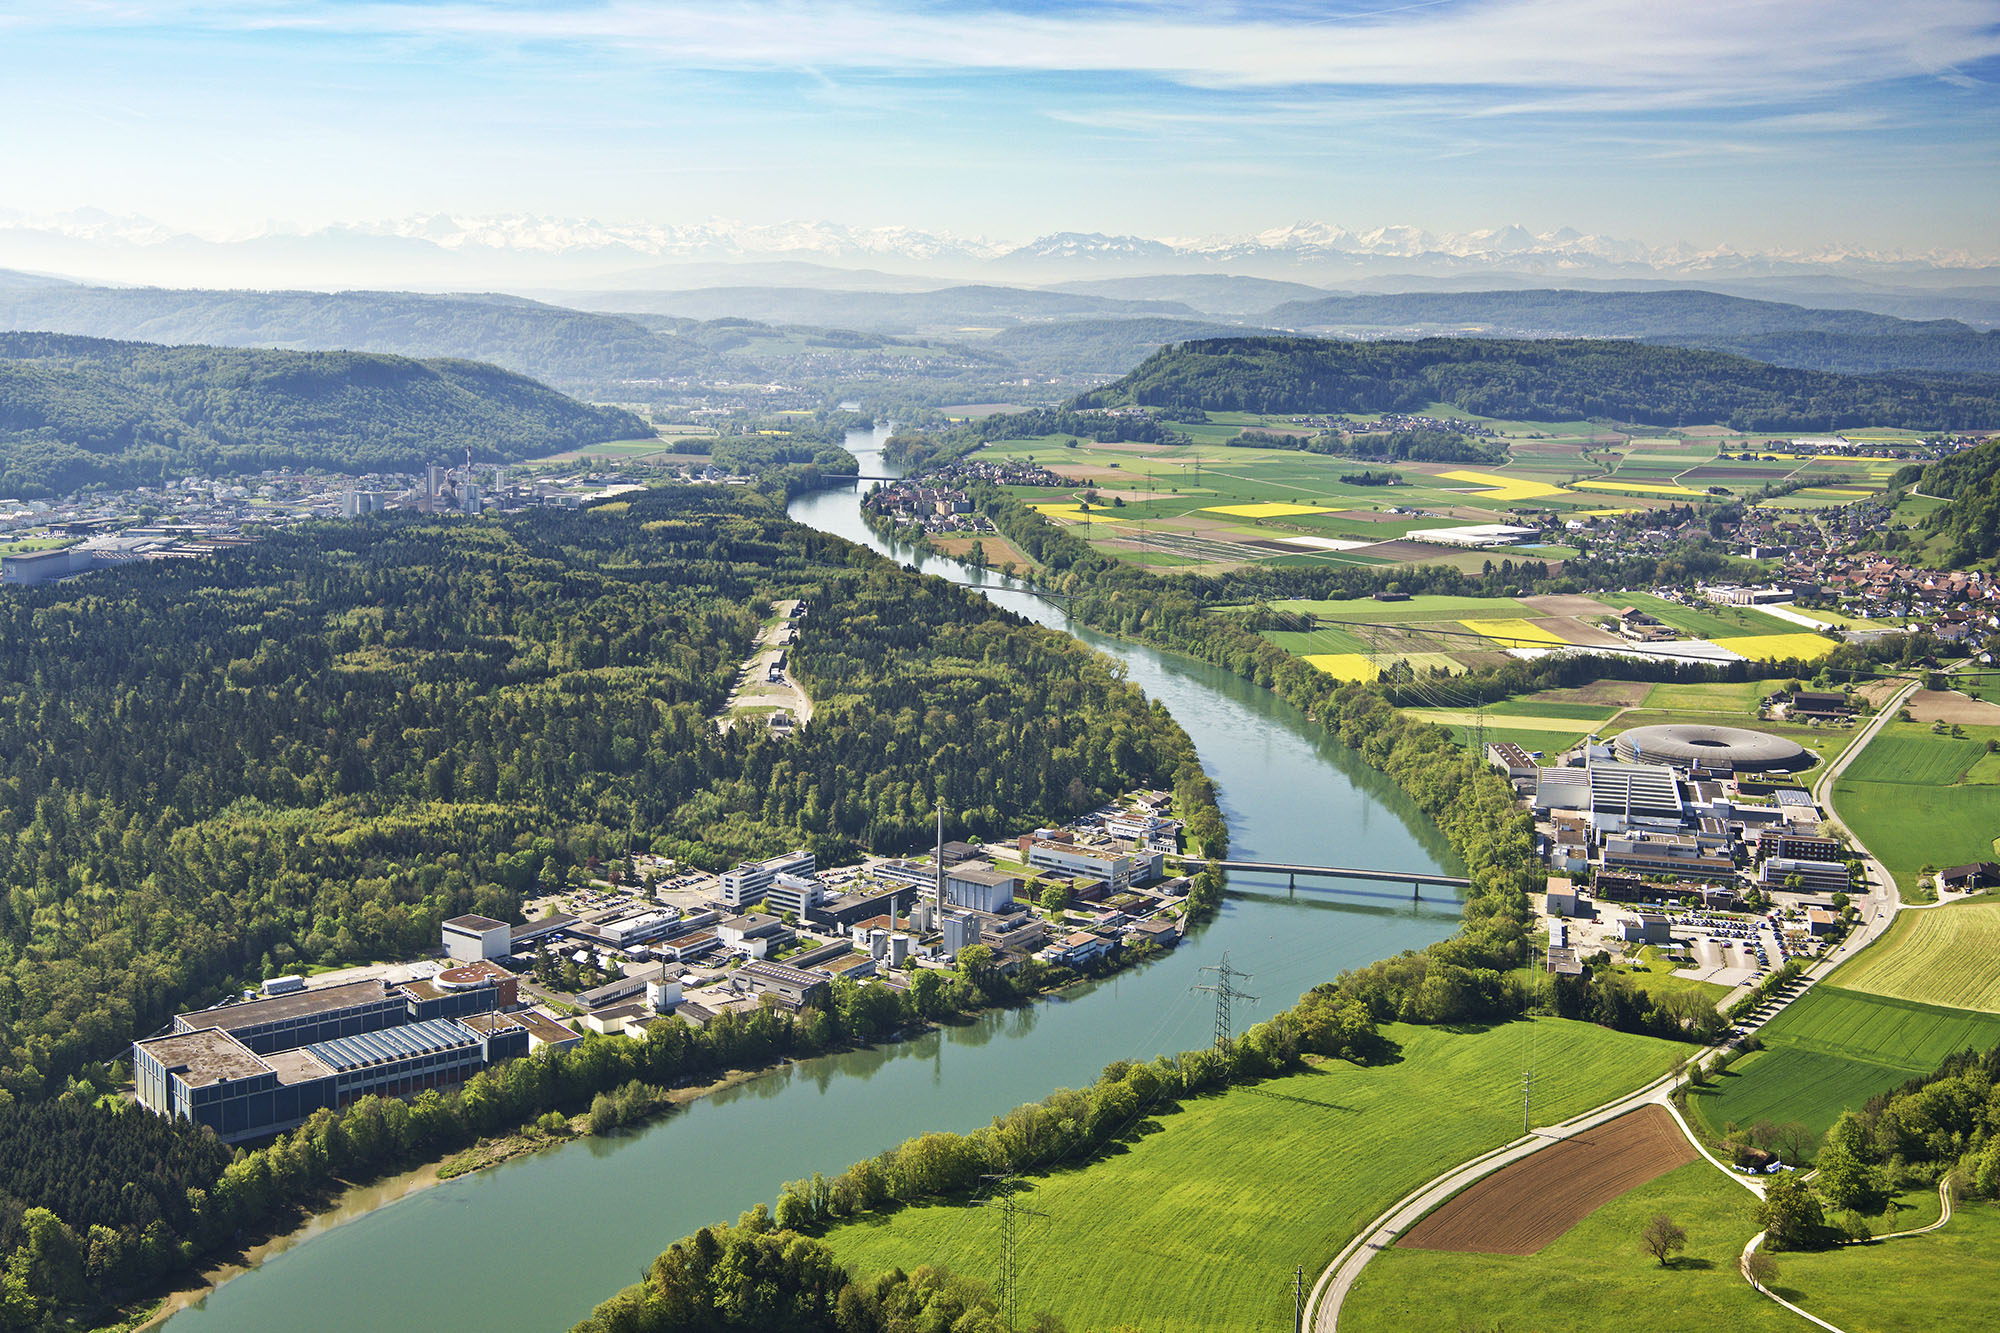
\includegraphics[height=0.5\textheight]{logos/PSI_helicopter}};
    \end{tikzpicture}
    
\begin{tikzpicture}
      \filldraw[fill=lightgray!40!white, draw = none] (0,0) rectangle (1,0.5\textheight);
    \end{tikzpicture}
  \end{adjustbox}
  \vspace{0.1cm}\\
  {\usebeamerfont{subtitle} \footnotesize \insertauthor\, ::  \insertinstitute}
  \vspace{0.4cm}
  {\usebeamerfont{title} \LARGE \inserttitle}\\
  \vspace{0.4cm}
  {\usebeamerfont{subtitle} \footnotesize \insertdate}\\
  \vfilll
  \null\hfill\tiny Contact: \url{\myEmail}
\end{frame}

% Table of contents slide, comment this block out to remove it.
%\begin{frame}[noframenumbering]
%\frametitle{Overview}
%\tableofcontents % Throughout your presentation, if you choose to use \section{} and \subsection{} commands, these will automatically be printed on this slide as an overview of your presentation.
%\end{frame}

%----------------------------------------------------------------------------------------
%	PRESENTATION SLIDES
%----------------------------------------------------------------------------------------

\section{Progress Report}
\begin{frame}
    \frametitle{Correctness of the Langevin Solver}

\begin{itemize}[label=$\bullet$]
    \item Solver only works if drag and diffusion is added (but is noisy) $\rightarrow$ Check parameters
    \item Stops working after 122 timesteps without Langevin Terms (similarly if only one of the collisional terms is added)
\end{itemize}

Possible Sources of Error:
\begin{itemize}[label=$\bullet$]
    \item Constant focusing can't contain accelerating particles
    \item Particles leave spatial and velocity Domain
    \item Wrong parameter set
\end{itemize}

\end{frame}

\begin{frame}
    \frametitle{GPU Compatibility}

\begin{itemize}[label=$\bullet$]
    \item Solver / Timestepping runs now on GPU
    \item Data Dumping still facing issues due to incorrect memory spaces
\end{itemize}

\end{frame}

\end{document} 
